%===============================================================================
% $Id: ifacconf.tex 19 2011-10-27 09:32:13Z jpuente $  
% Template for IFAC meeting papers
% Copyright (c) 2007-2008 International Federation of Automatic Control
%===============================================================================
\documentclass{ifacconf}

\usepackage{graphicx}      % include this line if your document contains figures
\usepackage{natbib}        % required for bibliography
\usepackage{subfigure}
%===============================================================================
\begin{document}
\begin{frontmatter}

\title{DORIS - A MOBILE ROBOT FOR INSPECTION AND MONITORING OF
OFFSHORE FACILITIES\thanksref{footnoteinfo}} 
% Title, preferably not more than 10 words.

\thanks[footnoteinfo]{This work is supported primarily by Petrobras S.A. and
Statoil Brazil Oil \& Gas Ltda under contract COPPETEC 0050.0079406.12.9
(ANP-Brazil R \& D Program), and in part by the Brazilian research agencies CNPq
and FAPERJ}

\author[First]{First A. Author} 
\author[Second]{Second B. Author, Jr.} 
\author[Third]{Third C. Author}
\author[Forth]{Forth D. Author}

\address[First]{Research and Development Center, Petrobras/CENPES, Rio de
Janeiro, Brazil} 
\address[Second]{Mathematical Sciences and Technology Department, Norwegian
University of Life Sciences, Oslo, Norwegian }
\address[Third]{Electrical
Engineering Department, COPPE UFRJ, Rio de Janeiro, Brazil, (e-mail: )}
\address[Forth]{TPD RD New Development Solutions, Statoil ASA}

\begin{abstract}                % Abstract of not more than 250 words.
DORIS is a research project which endeavors to design and implement a mobile
robot for remote supervision, diagnosis, and data acquisition on offshore
facilities. The proposed system is composed of a railguided robot capable of
carrying different sensors through the inspected area. This paper presents a
general overview of the robot and a description of the developed software
architecture, embedded electronics and power supply system. Initial results
with teleoperational navigation validate the concepts considered so far and
rise several challenges in the three fields.
\end{abstract}

\begin{keyword}
Mobile robots; Field robotics; Decurity and safety of HMS.
\end{keyword}

\end{frontmatter}
%===============================================================================

\section{Introduction}
Safety and efficient operation are imperative factors to offshore production
sites and a main concern to all Oil \& Gas companies. A promising solution to
improve both safety and efficiency is to increase the level of automation on
the platforms by introducing robotic systems.

During the last decade, several Oil \& Gas companies, research groups, and
academic communities have shown an increasing interest in the use of robots for
operation on offshore facilities.  

Recent studies project a substantial decrease in the level of human operation
and an increase in automation on future offshore oil fields
~\cite{skourup2009robotized}.The studies also point out the potential increase
in efficiency and productivity with robot operators, besides the improvement of
Health, Safety, and Environment (HSE) conditions, as robots can replace humans
in tasks performed in unhealthy, hazardous, and confined areas ~\cite{pal}. 
In~\cite{abb}, it is considered the use of robots in Oil \& Gas facilities in
operations that require both high precision and strength, regardless of weather conditions.

In the specific case of Brazil, the Oil \& Gas industry is growing at a high
pace, mainly due to the recent discoveries of big oil fields in the pre-salt
layer off the Brazilian coast. These oil reservoirs are located farther than
300 km from the shore and at depths of 5000 to 7000 km. These factors,
especially the large distances, motivate the development of an offshore
production system with a high degree of automation based on advanced robotics
systems.

Among the research groups interested in offshore robotics, \emph{Fraunhofer
IPA} is pioneer in proposing and demonstrating the applicability of mobile
robots for offshore inspection and maintenance tasks \emph{in
loco} ~\cite{mimroex2}. One example is MIMROex ~\cite{mimroex}, capable of
navigating safely, building maps, and executing inspection tasks autonomously
throughout the topside of platforms.

Another robotic device applied in offshore environments is Sensabot
~\cite{sensabot}, capable of safely inspect and monitor hazardous and remote
production facilities. The robot can sustain high temperatures, is able to
reach areas with difficult access, and is certified to operate in explosive and
toxic environments.

SINTEF-ICT is another group interested in manipulators applied to the oil and
gas industry. Inspection and maintenance operations in a simulated production
process are performed by the cooperation of a gantry-mounted manipulator and a
floor-mounted robot ~\cite{kyrkjebo2009robotic}.

In this paper, we describe the DORIS project, which aims to develop a mobile
robot to perform monitoring, inspection, and simple intervention tasks in an
offshore platform. To this end, the system must be able to move throughout the
monitored environment carrying different sensors, analyzing sensor data
\emph{in loco} or storing it for a posterior analysis, and interpreting the
results. The sensors can identify abnormalities such as intruders in restricted
areas, abandoned objects, smoke, fire, and liquid and gas leakages.
Furthermore, the robot is able to make machinery diagnosis, read instruments,
and perform interventions on valves and other equipment using an embedded manipulator.

The paper is organized as follows: a general overview of the robot and its main
challenges are presented in Section \ref{sec:general_overview}, detailed
descriptions of the software architecture, embedded electronics and power supply
system are taken in Sections \ref{sec:software_overview},
\ref{sec:electronics_overview} and \ref{sec:powersupply_overview} respectively.
In Section \ref{sec:results}, preliminary results are shown, and concluding
remarks are drawn in Section \ref{sec:conclusions}. 

% Please stick to the format defined by the \texttt{ifacconf} class, and
% do not change the margins or the general layout of the paper. It
% is especially important that you do not put any running header/footer
% or page number in the submitted paper.\footnote{
% This is the default for the provided class file.}
% Use \emph{italics} for emphasis; do not underline.
% 
% Page limits may vary from conference to conference. Please observe the 
% page limits of the event for which your paper is intended.


\section{General Overview}\label{sec:general_overview}

The proposed system is composed of a robot with cameras, microphones, gas,
vibration and temperature sensors, and a manipulator arm. The robotic device is
guided by a rail and both the robot and the rail follows a modularity concept.
Additional robot modules can be annexed to include other sensors, and the rail
track can be modified by adding or replacing rail segments, thus enabling
operation in different areas of the platform.% Robot modules are organized by
% functionality, for example, traction and sensing modules.

The robot will be controlled autonomously or by teleoperation. Task managing
can be either in automatic (programmed using a mission interface) or manual
mode (real-time remote operation). The teleoperation and monitoring
capabilities guarantee online access to the embedded sensors, providing
information about the surrounding environment and the robot operating
conditions with real-time processing. Figure~\ref{fig:DORIS-overview}
illustrates the operation in a production plant.

%\begin{figure} [!h]
%    \begin{center}
%    \includegraphics[width=8.8cm]{figs/DORIS_overview.jpg}  % width is 8.4 cm.
%    \caption{Illustration of the DORIS robot operating in a platform topside environment}
%    \label{fig:DORIS-overview}
%    \end{center}
%\end{figure}

\begin{figure}[ht]
\centering
\subfigure[Robot's operational scenario in a production plant]{%
    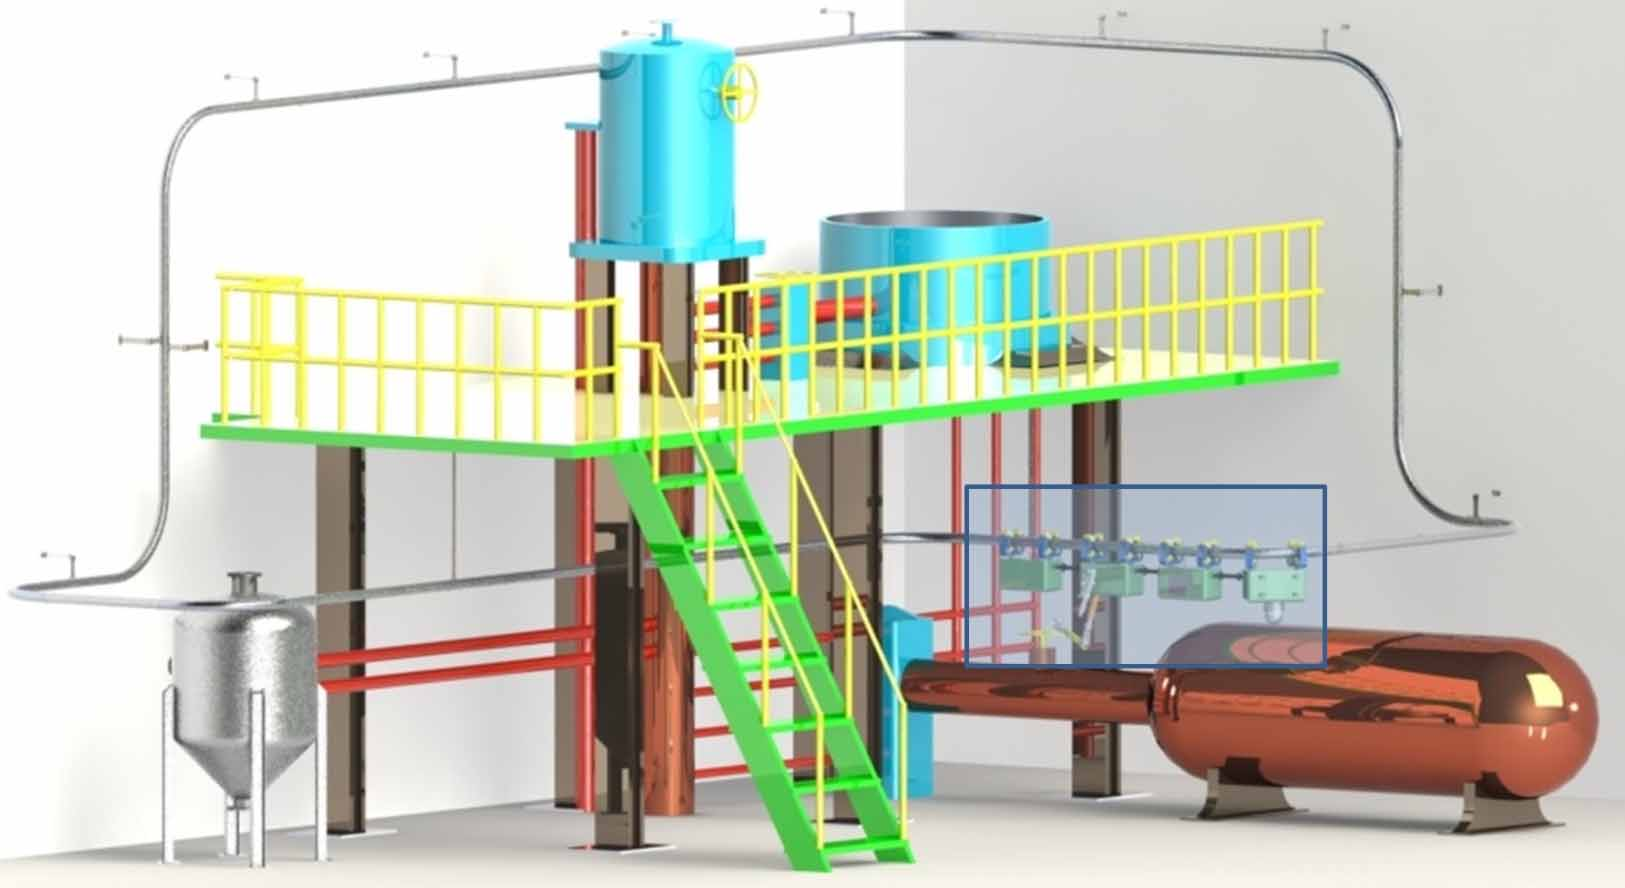
\includegraphics[width=8.4cm]{figs/cenario1.jpg}  % width is 7.6 cm.
    \label{fig:cenario1}} 
\subfigure[Detailed zoom of the robot]{%
    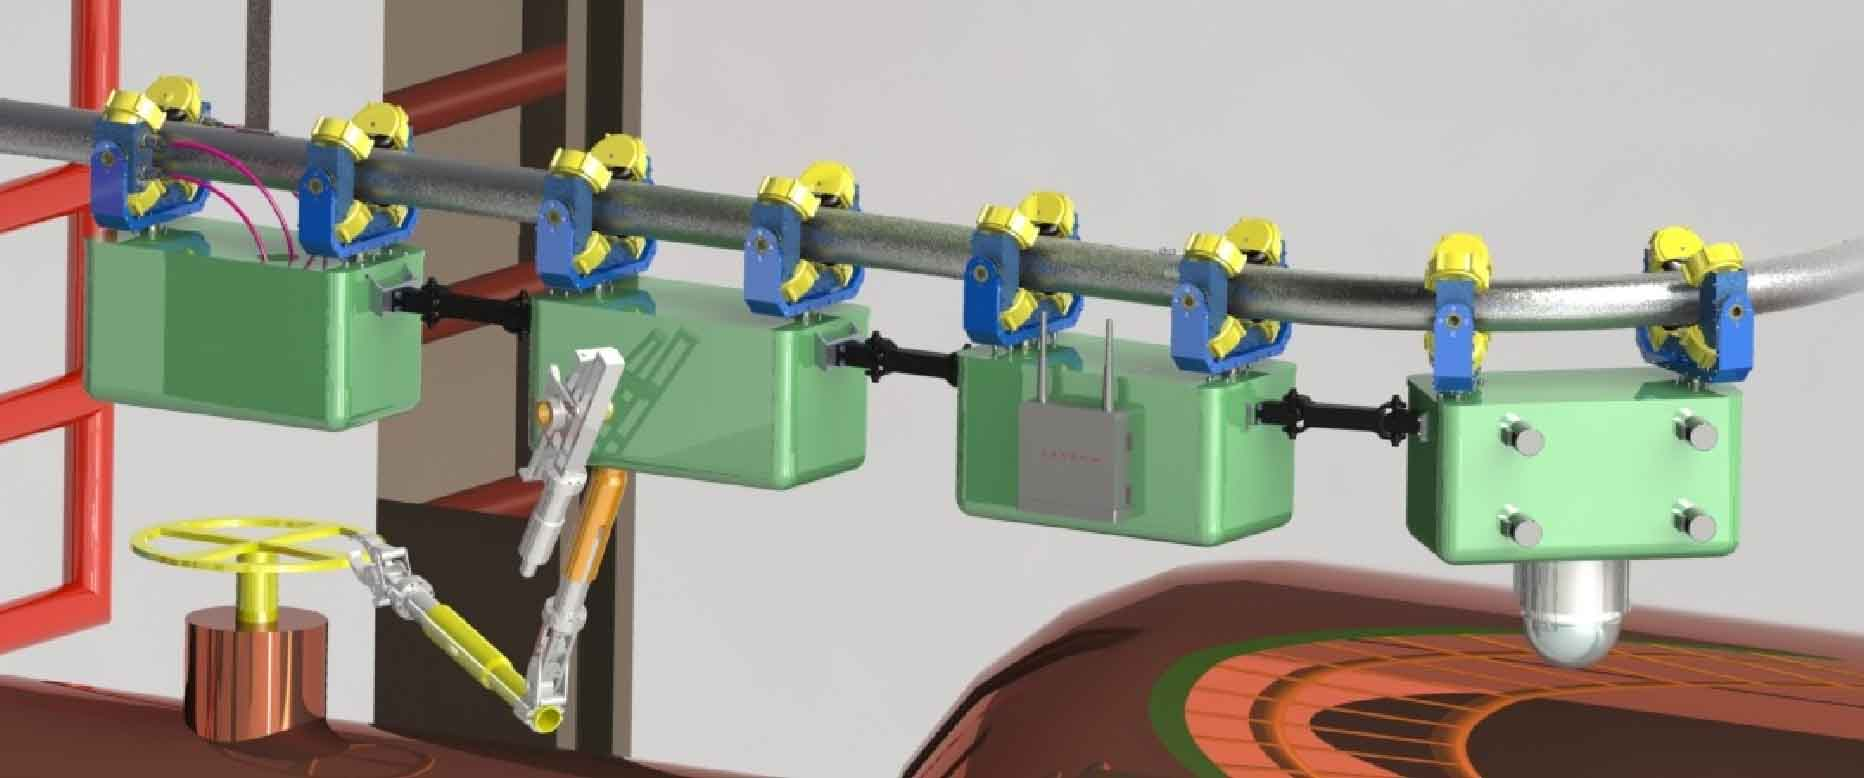
\includegraphics[width=8.4cm]{figs/zoom.jpg}  % width is 7.6 cm.
    \label{fig:zoom}}\vspace{-.1cm}
\caption{Illustration of the DORIS robot operating in a production plant.}\vspace{-0.25cm}
\label{fig:DORIS-overview}
\end{figure}

The DORIS project can be divided into five subsystems: electronics, power
supply, software, mechanics and signal processing.

%-------------------------------------------------------------------------------------------------------------------------
%ELECTRONICS
%-------------------------------------------------------------------------------------------------------------------------
The electronics subsystem is responsible for providing embedded computational
support for the robot control, signal processing, task managing, and local and
remote communication. The device motion is controlled through drivers that can
receive position, velocity, or current setpoints. The embedded electronics has
two printed circuit boards for the vehicle support system: energy distribution
and monitoring, basic failure detection, emergency handling and devices'
control.
% (EPOS from Maxon Motors)

%Concerning robustness and safety required to operate in harsh environments, the robot  must be sealed against water and ingress of objects, resistant to a wide temperature range, protected from impact and vibration, electrically protected to avoid explosion by ignition, and equipped with a monitoring system.%protected 2x?

%-------------------------------------------------------------------------------------------------------------------------
%POWER SUPPLY
%-------------------------------------------------------------------------------------------------------------------------
The power supply system uses military-class lithium-ion batteries, which have
small size and high energy capacity. In the first prototype of DORIS, four
batteries are used to power the motors and two to power the other electronics
components. 

%Considering the requirements to operate in harsh environments and classified areas,

%-------------------------------------------------------------------------------------------------------------------------
%SOFTWARE
%-------------------------------------------------------------------------------------------------------------------------
The main objective of the software subsystem is to allow the implementation of
high- and low-level control of the robot. The tools used to develop DORIS
software architecture must consider two important factors: they have to be
commercially available, and provide modular functionalities. These requirements
led to the adoption of Qt as the graphical interface framework ~\cite{qt},
Robot Operating System (ROS) as the communication middleware ~\cite{ros}, and
Ubuntu as the operating system.

%Robots may be very complex, so it is important to divide this complexity into smaller, independent parts.

The software provides autonomous control (programmed tasks) and remote control
through a Graphical User Interface (GUI) in the Host Control Base (HCB)
computer. The HCB is composed of a set of processes running in parallel
denominated ROS nodes, which can communicate with each other. To deal with this
environment, a new software architecture called Robot Package Software is
proposed, dividing the software into tools (graphical windows) and components
(processing and communication unities), and grouping them into a dynamic
library. %A DORIS Package is developed as a library containing a list of components and tools for the DORIS robot.

%Firstly, the robot needs to perform the task it is set to do and do so in the safest and most efficient way. This may include the control of the robot and machine learning algorithms. The software also needs to be suited for low-level control of the various components when this is not embedded.

%-------------------------------------------------------------------------------------------------------------------------
%Mechanics
%-------------------------------------------------------------------------------------------------------------------------
The mechanical project designs the rail, the
traction and passive modules, and the joints used to couple them. The design
allows the robot to move smoothly in a 3D space and makes full stop anywhere
on the rail. Considering the severe corrosion and weather conditions in
offshore environments, the choice of materials are imperative to the success of
the project and certified solutions must be considered.

The robot is composed of two modules at its default configuration, but it is
conceived so that other modules can be added. The total weight of this
configuration is estimated at 50 kg and we expect to have a maximum speed of
1m/s.

The design incorporates the use of gimbals with wheels as guides for
the module on the rail. The motors are fixed on the gimbal and transmit its
torque to the wheels via spur gears. The use of gimbals is an proper choice
concerning stability, guidance, and support. Furthermore, it is possible to have
a smooth vertical motion applying radial forces by the clamping mechanism.


%-------------------------------------------------------------------------------------------------------------------------
%OTHER CHALLENGES
%-------------------------------------------------------------------------------------------------------------------------
Considering the robot functionalities and the aggressive offshore environment,
several challenges should be addressed. Temperatures in offshore facilities can
vary between $-30^{\circ}$C to $50^{\circ}$C, relative humidity can reach
100\%, and there may be splash water, salty air, storms, and high extensive
corrosion ~\cite{graf2007mobile}. 

Concerning robustness and safety required to operate in classified areas, the
robot must be sealed against water and objects, resistant to a wide temperature
range, protected from impact and vibration, electrically shielded to avoid
explosion by ignition, and equipped with a monitoring system.

%{\color{red}Moreover, the robot parts must have special enclosures to turn it explosion-proof and allow operation in classified areas.}

Another challenge is that the embedded computers must run heavy signal
processing algorithms, requiring high computational power. However, the power
supply subsystem must efficiently provide power and maintain a low level of
power consumption.

Further complications arise because the system is designed to move in confined
areas and have efficient wireless communication with operators, providing
online information of sensors data. Finally, the robot must have a modular and
flexible design, employing plug and play extensions.%, which represents an
% additional complication.%challenge?

\subsection{Review Stage}

For submission guidelines, follow instructions on paper submission
system as well as the event website.

Note that conferences impose strict page limits, so it will be better
for you to prepare your initial submission in the camera ready layout
so that you will have a good estimate for the paper
length. Additionally, the effort required for final submission will be
minimal.

\subsection{Equations}

Some words might be appropriate describing equation~(\ref{eq:sample}), if 
we had but time and space enough. 

\begin{equation} \label{eq:sample}
{{\partial F}\over {\partial t}} = D{{\partial^2 F}\over {\partial x^2}}.
\end{equation}

\subsubsection{Example.} This equation goes far beyond the
celebrated theorem ascribed to the great Pythagoras by his followers.

\begin{thm}   % use the thm environment for theorems
The square of the length of the hypotenuse of a right triangle equals
the sum of the squares of the lengths of the other two sides.
\end{thm}

\begin{pf}    % and the pf environment for proofs
The square of the length of the hypotenuse of a right triangle equals the sum of the squares 
of the lengths of the other two sides.
\end{pf}

%% There are a number of predefined theorem-like environments in
%% ifacconf.cls:
%%
%% \begin{thm} ... \end{thm}            % Theorem
%% \begin{lem} ... \end{lem}            % Lemma
%% \begin{claim} ... \end{claim}        % Claim
%% \begin{conj} ... \end{conj}          % Conjecture
%% \begin{cor} ... \end{cor}            % Corollary
%% \begin{fact} ... \end{fact}          % Fact
%% \begin{hypo} ... \end{hypo}          % Hypothesis
%% \begin{prop} ... \end{prop}          % Proposition
%% \begin{crit} ... \end{crit}          % Criterion

Of course LaTeX manages equations through built-in macros. You may
wish to use the \texttt{amstex} package for enhanced math
capabilities.

\subsection{Figures}

To insert figures, use the \texttt{graphicx} package. Although other
graphics packages can also be used, \texttt{graphicx} is simpler to
use. See  Fig.~\ref{fig:bifurcation} for an example.

\begin{figure}
\begin{center}
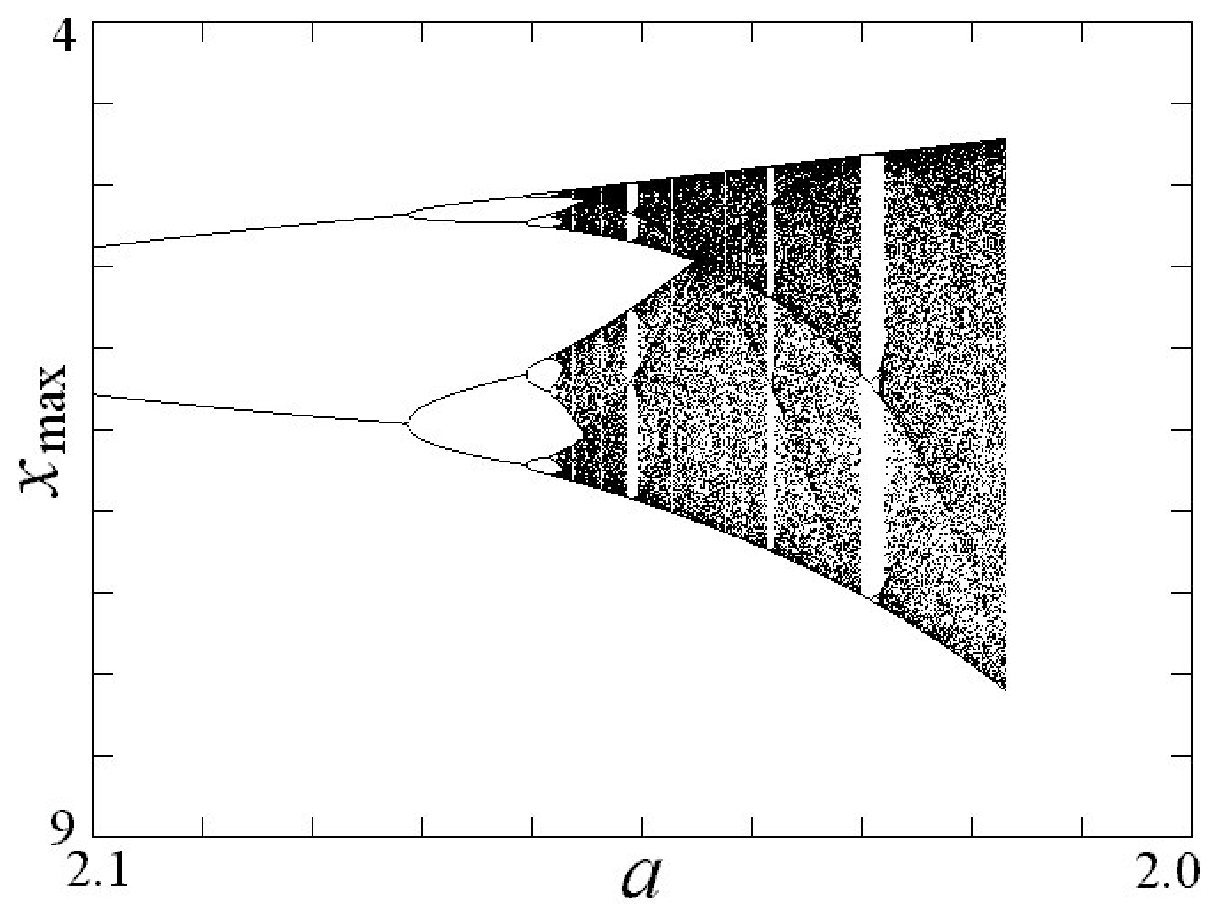
\includegraphics[width=8.4cm]{bifurcation}    % The printed column width is 8.4 cm.
\caption{Bifurcation: Plot of local maxima of $x$ with damping $a$ decreasing} 
\label{fig:bifurcation}
\end{center}
\end{figure}

Figures must be centered, and have a caption at the bottom. 

\subsection{Tables}
Tables must be centered and have a caption above them, numbered with
Arabic numerals. See table~\ref{tb:margins} for an example.

\begin{table}[hb]
\begin{center}
\caption{Margin settings}\label{tb:margins}
\begin{tabular}{cccc}
Page & Top & Bottom & Left/Right \\\hline
First & 3.5 & 2.5 & 1.5 \\
Rest & 2.5 & 2.5 & 1.5 \\ \hline
\end{tabular}
\end{center}
\end{table}

\subsection{Final Stage}

Authors are expected to mind the margins diligently.  Papers need to
be stamped with event data and paginated for inclusion in the
proceedings. If your manuscript bleeds into margins, you will be
required to resubmit and delay the proceedings preparation in the
process.

\subsubsection{Page margins.} See table~\ref{tb:margins} for the
page margins specification. All dimensions are in \emph{centimeters}.


\subsection{PDF Creation}

All fonts must be embedded/subsetted in the PDF file. Use one of the
following tools to produce a good quality PDF file:

\subsubsection{PDFLaTeX} is a special version of LaTeX by Han The
Thanh which produces PDF output directly using Type-1 fonts instead of
the standard \texttt{dvi} file. It accepts figures in JPEG, PNG, and PDF
formats, but not PostScript. Encapsulated PostScript figures can be
converted to PDF with the \texttt{epstopdf} tool or with Adobe Acrobat
Distiller.

\subsubsection{Generating PDF from PostScript} is the classical way of
producing PDF files from LaTeX. The steps are:

\begin{enumerate}
  \item Produce a \texttt{dvi} file by running \texttt{latex} twice.
  \item Produce a PostScript (\texttt{ps}) file with \texttt{dvips}.
  \item Produce a PDF file with \texttt{ps2pdf} or Adobe Acrobat
  Distiller.
\end{enumerate}

\subsection{Copyright Form}

IFAC will put in place an electronic copyright transfer system in due
course. Please \emph{do not} send copyright forms by mail or fax. More
information on this will be made available on IFAC website.


\section{Units}

Use SI as primary units. Other units may be used as secondary units
(in parentheses). This applies to papers in data storage. For example,
write ``$15\,\mathrm{Gb}/\mathrm{cm}^2$ ($100\,\mathrm{Gb}/\mathrm{in}^2$)''. 
An exception is when
English units are used as identifiers in trade, such as ``3.5 in
disk drive''. Avoid combining SI and other units, such as current in
amperes and magnetic field in oersteds. This often leads to confusion
because equations do not balance dimensionally. If you must use mixed
units, clearly state the units for each quantity in an equation.  The
SI unit for magnetic field strength $\mathbf{H}$ is $\mathrm{A}/\mathrm{m}$. However, if you wish to
use units of $\mathrm{T}$, either refer to magnetic flux density $\mathbf{B}$ or
magnetic field strength symbolized as $\mu_0\,\mathbf{H}$. Use the center dot to
separate compound units, e.g., ``$\mathrm{A} \cdot \mathrm{m}^2$''.

\section{Helpful Hints}

\subsection{Figures and Tables}

Figure axis labels are often a source of confusion. Use words rather
than symbols. As an example, write the quantity ``Magnetization'', or
``Magnetization M'', not just ``M''. Put units in parentheses. Do not
label axes only with units.  For example, write ``Magnetization
($\mathrm{A}/\mathrm{m}$)'' or ``Magnetization ($\mathrm{A} \mathrm{m}^{-1}$)'', not just
 ``$\mathrm{A}/\mathrm{m}$''. Do not
label axes with a ratio of quantities and units. For example, write
``Temperature ($\mathrm{K}$)'', not ``$\mbox{Temperature}/\mathrm{K}$''.

Multipliers can be especially confusing. Write ``Magnetization
($\mathrm{kA}/\mathrm{m}$)'' or ``Magnetization ($10^3 \mathrm{A}/\mathrm{m}$)''. Do not write
``Magnetization $(\mathrm{A}/\mathrm{m}) \times 1000$'' because the reader would not know
whether the axis label means $16000\,\mathrm{A}/\mathrm{m}$ or $0.016\,\mathrm{A}/\mathrm{m}$.

\subsection{References}

Use Harvard style references (see at the end of this document). With
\LaTeX, you can process an external bibliography database 
using \texttt{bibtex},\footnote{In this case you will also need the \texttt{ifacconf.bst}
file, which is part of the \texttt{ifaconf} package.}
or insert it directly into the reference section. Footnotes should be avoided as
far as possible.  Please note that the references at the end of this
document are in the preferred referencing style. Papers that have not
been published should be cited as ``unpublished''.  Capitalize only the
first word in a paper title, except for proper nouns and element
symbols.

\subsection{Abbreviations and Acronyms}

Define abbreviations and acronyms the first time they are used in the
text, even after they have already been defined in the
abstract. Abbreviations such as IFAC, SI, ac, and dc do not have to be
defined. Abbreviations that incorporate periods should not have
spaces: write ``C.N.R.S.'', not ``C. N. R. S.'' Do not use abbreviations
in the title unless they are unavoidable (for example, ``IFAC'' in the
title of this article).

\subsection{Equations}

Number equations consecutively with equation numbers in parentheses
flush with the right margin, as in (\ref{eq:sample}).  To make your equations more
compact, you may use the solidus ($/$), the $\exp$ function, or
appropriate exponents. Use parentheses to avoid ambiguities in
denominators. Punctuate equations when they are part of a sentence, as
in

\begin{equation} \label{eq:sample2}
\begin{array}{ll}
\int_0^{r_2} & F (r, \varphi ) dr d\varphi = [\sigma r_2 / (2 \mu_0 )] \\
& \cdot \int_0^{\inf} exp(-\lambda |z_j - z_i |) \lambda^{-1} J_1 (\lambda  r_2 ) J_0 (\lambda r_i ) d\lambda 
\end{array}
\end{equation}

Be sure that the symbols in your equation have been defined before the
equation appears or immediately following. Italicize symbols ($T$
might refer to temperature, but T is the unit tesla). Refer to
``(\ref{eq:sample})'', not ``Eq. (\ref{eq:sample})'' or ``equation
(\ref{eq:sample})'', except at the beginning of a sentence: ``Equation
(\ref{eq:sample}) is \ldots''.

\subsection{Other Recommendations}

Use one space after periods and colons. Hyphenate complex modifiers:
``zero-field-cooled magnetization''. Avoid dangling participles, such
as, ``Using (1), the potential was calculated'' (it is not clear who or
what used (1)). Write instead: ``The potential was calculated by using
(1)'', or ``Using (1), we calculated the potential''.

A parenthetical statement at the end of a sentence is punctuated
outside of the closing parenthesis (like this). (A parenthetical
sentence is punctuated within the parentheses.) Avoid contractions;
for example, write ``do not'' instead of ``don' t''. The serial comma
is preferred: ``A, B, and C'' instead of ``A, B and C''.


\section{Conclusion}

A conclusion section is not required. Although a conclusion may review
the main points of the paper, do not replicate the abstract as the
conclusion. A conclusion might elaborate on the importance of the work
or suggest applications and extensions.

\begin{ack}
Place acknowledgments here.
\end{ack}

\bibliography{ifacconf}             % bib file to produce the bibliography
                                                     % with bibtex (preferred)
                                                   
%\begin{thebibliography}{xx}  % you can also add the bibliography by hand

%\bibitem[Able(1956)]{Abl:56}
%B.C. Able.
%\newblock Nucleic acid content of microscope.
%\newblock \emph{Nature}, 135:\penalty0 7--9, 1956.

%\bibitem[Able et~al.(1954)Able, Tagg, and Rush]{AbTaRu:54}
%B.C. Able, R.A. Tagg, and M.~Rush.
%\newblock Enzyme-catalyzed cellular transanimations.
%\newblock In A.F. Round, editor, \emph{Advances in Enzymology}, volume~2, pages
%  125--247. Academic Press, New York, 3rd edition, 1954.

%\bibitem[Keohane(1958)]{Keo:58}
%R.~Keohane.
%\newblock \emph{Power and Interdependence: World Politics in Transitions}.
%\newblock Little, Brown \& Co., Boston, 1958.

%\bibitem[Powers(1985)]{Pow:85}
%T.~Powers.
%\newblock Is there a way out?
%\newblock \emph{Harpers}, pages 35--47, June 1985.

%\bibitem[Soukhanov(1992)]{Heritage:92}
%A.~H. Soukhanov, editor.
%\newblock \emph{{The American Heritage. Dictionary of the American Language}}.
%\newblock Houghton Mifflin Company, 1992.

%\end{thebibliography}

\appendix
\section{A summary of Latin grammar}    % Each appendix must have a short title.
\section{Some Latin vocabulary}              % Sections and subsections are supported  
                                                                         % in the appendices.
\end{document}
